\chapter{Planning integration}

This chapter aims to \textbf{integrate} the planning part developed by \textit{Filippo Rossi}\footnote{His entire project is described in \autoref{sub:planning}} \cite{fr}. What already discussed in the previous chapters leads to a \textbf{working} version of the robot (it is able to move around), but does not have any practical use, because you need to set \textbf{where} you want the robot to go \textbf{every time}. This is the goal of this chapter: add some \textbf{missions control} (?), to give the robot some tasks it has to complete, without the needing of any \textbf{low-level human interaction}. Everything except the custom service messages can be found in \code{planning\_bridge} package in Figure (?).

\section{Modifications from original planning}

When the planning was developed, Filippo could not receive any feedback, since we were facing some other challenges (i.e. make robots move autonomously). So, in response, the planning is more like a \textbf{generic workspace} to which we can add some \textbf{modifications} to meet our specific needs; then we can attach the \textbf{adapted workspace} to what was already developed, since \acrshort{ros} is \textbf{modular}.

% aggiungere entrance tag per entrata porta, dato che non è ben definita

\subsection*{Change JSON structure}
\label{sub:json}

Since that JSON file was written as a \textbf{list of dictionaries}, it would be required to iterate \textbf{over every element} and search for the one with the \textbf{requested name}, and when they match, it is possible to get the coordinates. Instead, for an easier use, a dictionary is created with the name of the room as \textbf{key} and the coordinates of that room center and boundaries as \textbf{value}. A before and after comparision (?) is shown in \autoref{lst:origjson} and \autoref{lst:modjson}. This operation has been performed with the \code{Python} script shown in \autoref{lst:script}.

\noindent\begin{minipage}{0.425\textwidth}
\noindent\begin{lstlisting}[
    language=json,
    style=jsonStile,
    caption={Original JSON structure},
    label={lst:origjson}]
[
    {
        "label": "povo_1_258",
        "center": [
            -11.749180327868853,
            -35.01639344262295,
            1.5
        ],
        "max": [
            -8.0,
            -30.5,
            1.5
        ],
        "min": [
            -15.5,
            -40.0,
            1.5
        ]
    },
    ...
]
\end{lstlisting}
\end{minipage}
\noindent\begin{minipage}{0.15\textwidth}
    \centering
    \noindent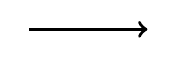
\begin{tikzpicture}
        \draw[->, very thick] (0,0) -- (1.5,0);
    \end{tikzpicture}
\end{minipage}
\noindent\begin{minipage}{0.425\textwidth}
\noindent\begin{lstlisting}[
    language=json,
    style=jsonStile,
    caption={Modified JSON structure},
    label={lst:modjson}]

{
    "povo_1_258": {
        "center": [
            -11.749180327868853,
            -35.01639344262295

        ],
        "max": [
            -8.0,
            -30.5

        ],
        "min": [
            -15.5,
            -40.0

        ]
    },
    ...
}
\end{lstlisting}
\end{minipage}


\subsection*{Correct waypoint coordinates}
\label{sub:waypoints}

Thanks to Filippo's \textbf{waypoints extractor} and \code{cvat} \textbf{annotation software}, all the coordinate information can be found in a \textbf{JSON file}: when the robot is told to move in a certain room, only step to take is \textbf{searching} its name in the file and reading its \textbf{coordinates}.
But the mesh, the same described in \autoref{sub:map}, used for generating those waypoints is not the same of the real environment, and navigation map is rotated with respect to this one.

Using \textit{Blender} \cite{blender}, after loading both mesh and map, some modifications that lead to a better result can be applied: by turning the mesh by \textbf{135 sexagesimal degrees counterclockwise} around the Z axis, scaling (up) the long side (Y axis) of the mesh \textbf{1.0925 times}, and translating 6.8210 meters along the short side (X axis) and \textbf{8.7180 meters} along the long side (Y axis). Luckily, when applying these transformations on the entire mesh you do it on its own points, and apply them on these waypoints in the JSON file is the same, without needing to repeat the annotation process from the beginning. These \textit{transformations} have been performed (?)
 with the Python script in \autoref{lst:script}

\applymulticoltrue

\noindent\begin{lstlisting}[
    language=Python,
    style=PythonStile,
    caption={Python script used to transform waypoint coordinates},
    label={lst:script}]
...
import numpy as np

translation = np.array([6.8210, 8.7180, 0])
rot_z = 135 * np.pi / 180
scale_y = 1.0925
...
rot_matrix = np.array(
    [[np.cos(rot_z), -np.sin(rot_z), 0],
     [np.sin(rot_z), np.cos(rot_z), 0],
     [0, 0, 1]])

scale_matrix = np.array([[1, 0, 0], 
                         [0, scale_y, 0],
                         [0, 0, 1]])

roto_scaling = np.dot(rot_matrix, scale_matrix)

# iterate over each element of the original list (original_data) and save all keys and values in a new dict (dict_data)
for obj in original_data:
    dict_data[obj["label"]] = {
        k: (-translation-np.dot(-roto_scaling, np.array(v)))[0:2].tolist()
        for k, v in obj.items()
        if k != "label"
    }
...
\end{lstlisting}

\applymulticolfalse

Rotation and scale matrices are calculated and fused together. Then(, as described in \autoref{sub:json},) the JSON structure is changed with dictionaries and each value of its corresponding key is transformed by applying the rotation-scale matrix and the translation vector. At the end, with \code{[0:2]}, only x and y coordinates are kept.

\subsection*{Remove stub nodes from execution}

Currently, the only actions supported are \code{ugv\_move} and \code{ugv\_transporting\_uav\_move}: although the name is different, they share the \textbf{same code} (they have been separated for planning reasons). For testing purposes, in the original planning some nodes were added to simulate \acrshort{ugv}s and \acrshort{uav}s: they were started at the beginning of the execution, but now these two have their real implementation, so the \textbf{stub ones} have been removed from the launch.

\section{Task executors} % creare launch file e splittare i due nodi (?) cambiare con nuovo setup (?)

Four nodes have been created to let the robot moves autonomously: 
\begin{itemize}
    \item \arguments{navigation client}{service and action client that sets the navigation goal when coordinates are received}
    \item \arguments{pose server}{service server responsible for returning the current pose of the robot when requested}
    \item \textbf{two planning clients} (\code{ugv\_move}\footnote{\label{fn:node}Node name is equal to action name} and \code{ugv\_transporting\_uav\_move}\footnoteref{fn:node}): \textit{action executor clients listening for next action to complete}
\end{itemize}

The entire workflow is shown in \autoref{fig:bridge}

\begin{figure}[h]
    \centering
    \begin{tikzpicture}
        \node [block] (plan-server) {PLANNING SERVER};
        \node [block, below=of plan-server] (nav-server) {NAVIGATION SERVER};
        \node [block, right=of plan-server] (plan-clients) {PLANNING CLIENTS};
        \node [block, right=of nav-server] (nav-client) {NAVIGATION CLIENT};
        \node [block, right=of plan-clients] (pose-server) {POSE SERVER};

        \draw [arrow] (plan-server) -- node [above] {plansys2\_msgs::msg} node [below] {::ActionExecution(?)} (plan-clients);
        \draw [arrow] (nav-client) -- node [above] {nav2\_msgs::action} node [below] {::NavigateToPose} (nav-server);
        \draw [arrow] (plan-clients.250) -- node [left] {float32 x, y} (nav-client.110);
        \draw [arrow] (nav-client.70) -- node [right] {bool success} (plan-clients.290);
        \draw [arrow] (plan-clients.6) -- (pose-server.174);
        \draw [arrow] (pose-server.186) -- node [below] {float32 x, y} (plan-clients.354);        
    \end{tikzpicture}
    \caption[Nodes interaction]{
        On the left, the already existing servers, in the center, the customized clients written, and on the right, the customized server written. On the arrows, the messages exchanged.
    }
    \label{fig:bridge}
\end{figure}

\subsection{Navigation client}

This node is both a \textbf{service server} and an \textbf{action client}: the first is used to receive the coordinates from the planning client and the second to connect to the navigation action server and set the just received destination. It is called only \textbf{once}, when a new task is created.

\subsection{Pose server}
\label{sub:pose}

When it receives a request, it returns the \textbf{current position} of the robot, which is \code{base\_link} position in the \code{map} frame. In order to achieve it, some other calculations need to be done: we are interested in \code{base\_link} frame, but the only transformation referring (to it) is the \code{odom} one, not the same used for waypoint coordinates. There is the need to express it from the \code{map} frame perspective, and luckily such a transformation (\code{map} $\rightarrow$ \code{odom}) is available thanks to \acrshort{amcl} node. 
Thanks to \code{tf\_echo} node \cite{tfexample} used as a template\footnote{If you follow the documentation, the process to get the transformation between two frames not directly connected, it will not work. The only node doing this and also working is \code{tf\_echo}.}, it was possible to obtain the correct transformation, \textbf{fusing} the required two.

\subsection{Planning clients}

%inserire immagine codice (?)

It is an \textbf{action client} (called \code{ActionExecutorClient}), coming from \code{plansys2\_executor} (cite (?)) package, of \code{plansys2\_msgs::action::ExecuteAction} action: it means that it connect to its server (called \code{ActionExecutor}) waiting for a \textbf{new goal} to reach. When it received a new goal is responsible for completing it, and at the same time he has to return \textbf{continuous feedback
} with the current percentage of completion, until the goal is \textbf{reached} (100\% completion).

When a new task has been created and started, the action server would call the \code{do\_work()} method of the designed client, to let it know a new job needs to be completed.
Inside this method the client transforms the \textbf{room name} (passed as goal) in \textbf{coordinates} and, if the goal was not already set, it passes it to the navigation client, making use of a custom service. After that, it asks \textbf{its current position} to the pose server (with another service) and uses it to set both the \textbf{initial and current position} (because the robot is not moving yet, the current position is the same as the initial one); using them, it returns a \textbf{percentage of completion} (0\%) to the action server.
This method, then, is called \textbf{continuously} until the task is completed to give some feedback: now the initial position is already set (and as a result also the goal), so it continues to ask for its current position (in order) to calculate the \textbf{euclidean distance} from the initial one and then, it returns a new percentage of completion. Because the path used to reach the destination might not be \textbf{a straight line} and the distance employed is the euclidean one, it could happen the current distance is \textbf{greater} than the initial one: in this case, they are swapped to keep 0\% as the \textbf{lower bound} of completion, otherwise it would become negative. Choosing the maximum between percentage of completion and zero would lead to \textbf{loss of information}, and it is the reason why it has not been used. 

$$ 1-\dfrac{current\_distance}{initial\_distance} $$ % inserire meglio formula con wrapfig (?)